\usetikzlibrary{arrows,chains,shapes,matrix,scopes,positioning,fadings,backgrounds,fit,mindmap,trees,decorations.markings,decorations.pathreplacing,calc}
\usetikzlibrary{decorations.pathmorphing,decorations.markings,trees,arrows.meta}

\definecolor{feeback}{rgb}{0,0.8,0} 
\definecolor{fepback}{rgb}{0,0.8,0} 
\definecolor{fepchip}{rgb}{0,0.9,0.9} 
\definecolor{sagback}{rgb}{0.9,0.9,0} 
\definecolor{sagchip}{rgb}{0,0.9,0.9} 
\definecolor{monitoring}{rgb}{1.,1.,1} 
\definecolor{fibercolor}{rgb}{0.9,0,0} 
\definecolor{locality}{rgb}{0,0.7,0.7} 
\tikzset{   
pics/.cd,   
disc/.style = {    
        code = {    
          \fill [white] ellipse [x radius = 1, y radius = 2/6]; 
     \path [left color = black!50, right color = black!50, middle color = black!25] 
      (-1+.05,-0.55) arc (180:360:1-.05 and 2/6-.05*2/6) -- cycle; 
     \path [top color = black!25, bottom color = white] (0,.05*2/3) ellipse [x radius = 1-.05, y radius = 2/6-.05*2/6]; 
     \path [left color = black!25, right color = black!25,middle color = white] (-1,0) -- (-1,-0.5) arc (180:360:1 and 2/6) -- (1,0) arc (360:180:1 and 2/6); 
     \foreach \r in {225,315} 
       \foreach \i [evaluate = {\s=30;}] in {0,2,...,30}
          \fill [black, fill opacity = 1/50]
             (0,0) -- (\r+\s-\i:1 and 2/6) -- ++(0,-0.5)
             arc (\r+\s-\i:\r-\s+\i:1 and 2/6) -- ++(0,0.5) -- cycle;
      \foreach \r in {45,135}
        \foreach \i [evaluate = {\s=30;}] in {0,2,...,30}
          \fill [black, fill opacity = 1/50]
             (0,0) -- (\r+\s-\i:1 and 2/6)
             arc (\r+\s-\i:\r-\s+\i:1 and 2/6)  -- cycle;
    }   },
  disc bottom/.style = {
    code = { 
     \foreach \i in {0,2,...,30}
        \fill [black, fill opacity = 1/60] (0,-0.55)
          ellipse [x radius = 1+\i/40, y radius = 2/6+\i/60];
      \path pic {disc};
    }   } }
\tikzstyle{vecArrow} = [thick, decoration={markings,mark=at position
   1 with {\arrow[semithick]{open triangle 60}}},
   double distance=3pt, shorten >= 5.5pt,
   preaction = {decorate},
   postaction = {draw,line width=1.4pt, white,shorten >= 4.5pt}]

\tikzstyle{fiber} = [thick, fibercolor]


\tikzset{
fee/.pic ={
	\draw [thick,fill=feeback]  (-0.275,-0.4) rectangle  (0.275,0.35);
	\draw[fill=black] (-0.18,0.25)  rectangle (-0.02,0.15);
	\draw[fill=black] (0.18,0.25)  rectangle (0.02,0.15);
	\draw[fill=black] (-0.18,0.1)  rectangle (-0.02,0.0);
	\draw[fill=black] (0.18,0.1)  rectangle (0.02,0.0);
	\draw (0,-0.2) node{\scriptsize FEE};
},
fep/.pic ={
	\draw [thick,fill=fepback]  (-0.3,-0.4) rectangle  (0.3,0.35);
	\draw[fill=fepchip] (-0.175,0.25)  rectangle (0.175,-0.1);
	\draw (0,-0.25) node{\scriptsize FEP};
},
sag/.pic ={
	\draw [thick,fill=sagback]  (-0.3,-0.4) rectangle  (0.3,0.35);
	\draw[fill=sagchip] (-0.125,0.2)  rectangle (0.125,-0.05);
	\draw (0,-0.25) node{\scriptsize SAG};
},
rack/.pic = {
	\draw [thick,rounded corners=4pt] (-1,2)  rectangle (0.5,-2);
	\draw [thick,rounded corners=2pt] (-0.9,1.9)  rectangle (0.4,1.6);
	\draw [thick,rounded corners=2pt] (-0.9,1.5)  rectangle (0.4,1.2);
	\draw [thick,rounded corners=2pt] (-0.9,1.1)  rectangle (0.4,0.8);
	\draw [thick,rounded corners=2pt] (-0.9,0.7)  rectangle (0.4,0.4);

	\draw [thick,rounded corners=2pt] (-0.9,0.3)  rectangle (0.4,0);
	\draw [thick,rounded corners=2pt] (-0.9,-0.1)  rectangle (0.4,-.4);
	\draw [thick,rounded corners=2pt] (-0.9,-.5)  rectangle (0.4,-0.8);
	\draw [thick,rounded corners=2pt] (-0.9,-0.9)  rectangle (0.4,-1.2);
	\draw [thick,rounded corners=2pt] (-0.9,-1.3)  rectangle (0.4,-1.6);
}, 
smallrack/.pic = {
	\draw [thick,rounded corners=2pt] (-1,2)  rectangle (0.5,-2);
	\draw [thick,rounded corners=1pt] (-0.9,1.9)  rectangle (0.4,1.6);
	\draw [thick,rounded corners=1pt] (-0.9,1.5)  rectangle (0.4,1.2);
	\draw [thick,rounded corners=1pt] (-0.9,1.1)  rectangle (0.4,0.8);
	\draw [thick,rounded corners=1pt] (-0.9,0.7)  rectangle (0.4,0.4);

	\draw [thick,rounded corners=1pt] (-0.9,0.3)  rectangle (0.4,0);
	\draw [thick,rounded corners=1pt] (-0.9,-0.1)  rectangle (0.4,-.4);
	\draw [thick,rounded corners=1pt] (-0.9,-.5)  rectangle (0.4,-0.8);
	\draw [thick,rounded corners=1pt] (-0.9,-0.9)  rectangle (0.4,-1.2);
	\draw [thick,rounded corners=1pt] (-0.9,-1.3)  rectangle (0.4,-1.6);
}, 
rackwfelix/.pic = {
	\draw [thick,rounded corners=4pt] (-1,2)  rectangle (1,-2);
	\draw [thick,rounded corners=2pt] (-0.9,1.9)  rectangle (0.9,1.0);
	\draw (-0.1,1.3) node {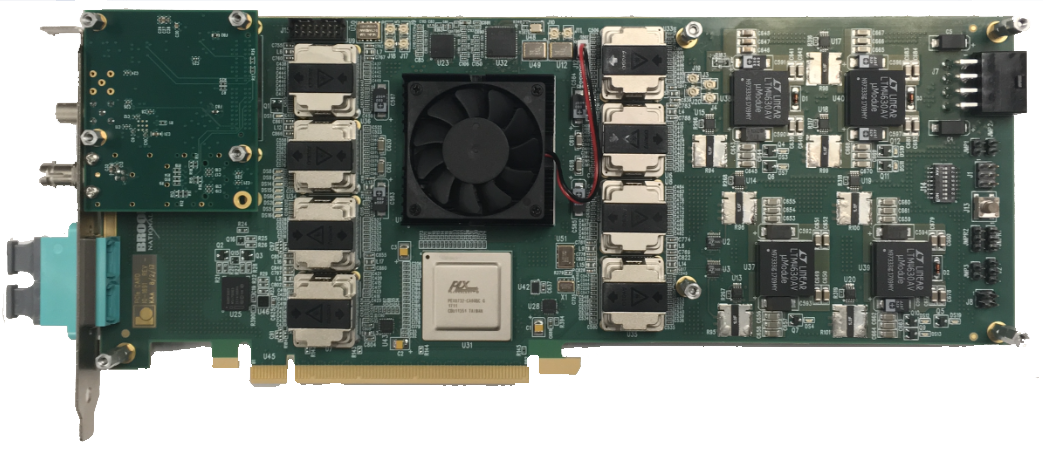
\includegraphics[width=1.5cm]{figs/felix.png}};
	\draw [thick,rounded corners=2pt] (-0.9,0.9)  rectangle (0.9,-0.1);
	\draw (-0.1,0.2) node {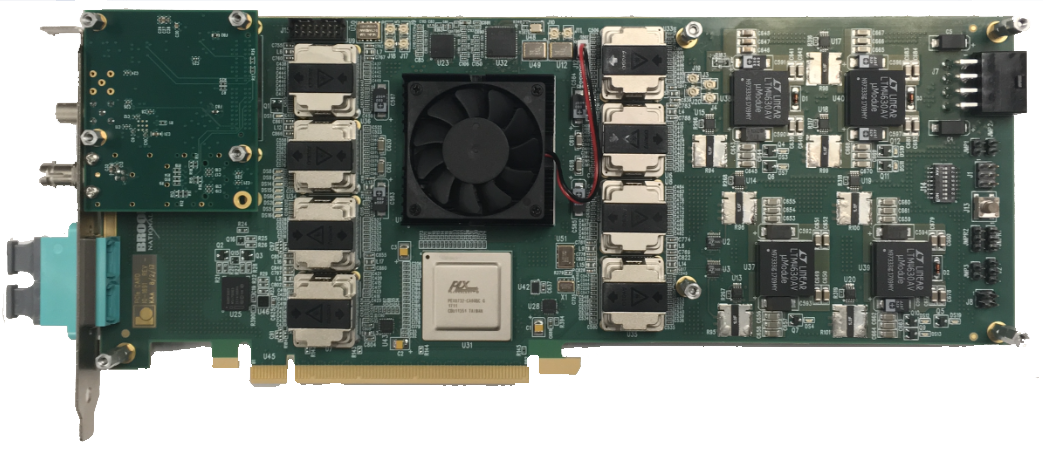
\includegraphics[width=1.5cm]{figs/felix.png}};
	\draw [thick,rounded corners=2pt] (-0.9,-.2)  rectangle (0.9,-1.2);
	\draw (-0.1,-0.9) node {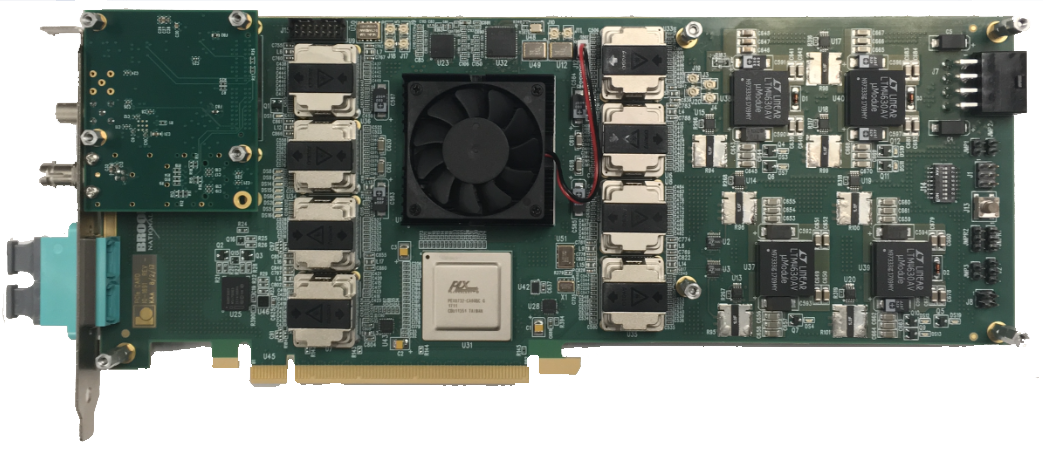
\includegraphics[width=1.5cm]{figs/felix.png}};
	\fill (-0.3,-1.6) circle(0.075);
	\fill (0,-1.6) circle(0.075);
	\fill (0.3,-1.6) circle(0.075);
}
}

{\sffamily
\begin{tikzpicture}     
  \draw (-3,0) node[]{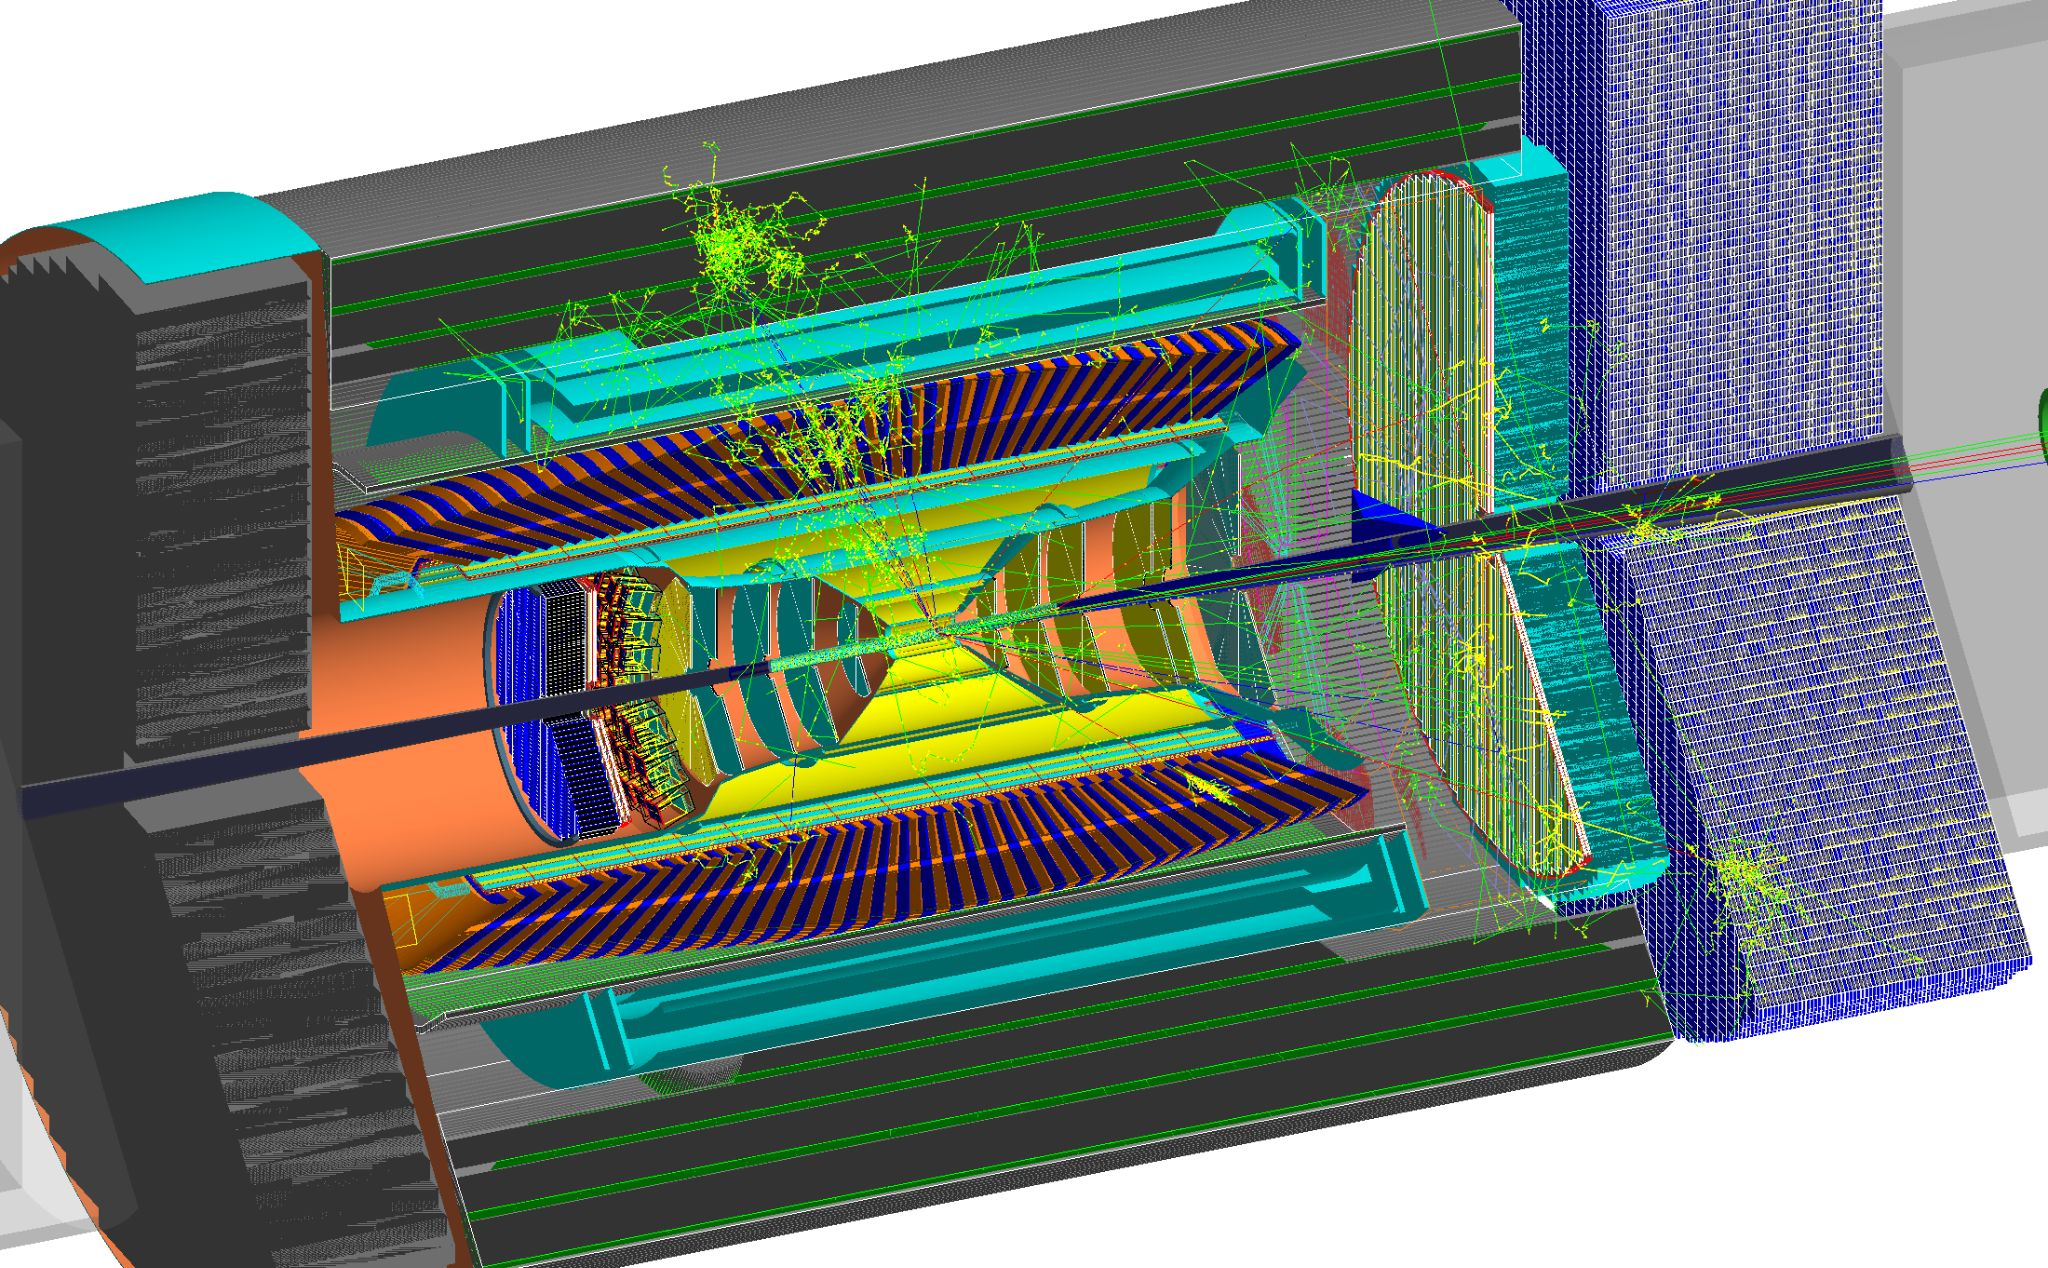
\includegraphics[width=3cm]{figs/detector.jpg}};   

\draw[locality] (-3,3) node {\large Detector};
\draw[locality] (1.5,3) node {\large Exp.~hall};
\draw[locality] (5.9,3) node {\large Counting room};
\draw[locality] (10.2,3) node {\large on-site/off-site};

\draw[locality,dashed,very thick] (-0.3,2.5) -- (-0.3,-5);
\draw[locality,dashed,very thick] (3.3,2.5) -- (3.3,-5);
\draw[locality,dashed,very thick] (8.3,2.5) -- (8.3,-5);



\draw[fiber] (-1.3,1.9) -- (4,1.9);
\draw[fiber] (-1.3,1.7) -- (4,1.7);
\draw[fiber] (-1.3,1.5) -- (4,1.5);
\draw[fiber] (-1.3,1.3) -- (4,1.3);

 \pic at ( -1.6 , 2.0) {fee};
 \pic at ( -1.4 , 1.8) {fee};
 \pic at ( -1.2, 1.6) {fee};
 \pic at ( -1 , 1.4) {fee};


\draw[fiber] (-1.3,0.2) -- (2.3,0.2);
\draw[fiber] (-1.3,0.) -- (2.3,0);
\draw[fiber] (-1.3,-.2) -- (2.3,-0.2);
\draw[fiber] (-1.3,-.4) -- (2.3,-.4);
\draw[fiber] (2.5,-0.1) -- (4,-0.1);
 \pic at ( -1.6 , 0.3) {fee};
 \pic at ( -1.4 , 0.1) {fee};
 \pic at ( -1.2, -0.1) {fee};
 \pic at ( -1 , -0.3) {fee};
  


\draw(-1.3,-1.5) -- (0.3,-1.5);
\draw(-1.3,-1.7) -- (0.3,-1.7);
\draw (-1.3,-1.9) -- (0.3,-1.9);
\draw(-1.3,-2.1) -- (0.3,-2.1);
  
\draw[fiber] (0.7,-1.6) -- (4,-1.6);
 \pic at ( -1.6 , -1.4) {fee};
 \pic at ( -1.4 , -1.6) {fee};
 \pic at ( -1.2,-1.8) {fee};
 \pic at ( -1 , -2) {fee};

\pic at (0.5,-1.75) {fep};

\pic at (2.5,-0.075) {sag};

\pic at (5,0) {rackwfelix};
\pic at (7.1,0) {rack};
\pic[scale=0.5] at (6.75,-3.05) {disc};
\draw  (6.75,-3.4) node[anchor=north]{\small Local buffer};
\draw[thick, rounded corners=3pt,fill=monitoring] (4,-4.6) rectangle (7.75,-5.4);
\draw (5.875,-5.) node {\small Monitoring};


\pic[scale=0.5] at (9.5,-0.6) {disc};
\pic[scale=0.5] at (9.5,-0.3) {disc};
\pic[scale=0.5] at (9.5,0.) {disc};
\pic[scale=0.5] at (9.5,0.3) {disc};
\pic[scale=0.5] at (9.5,0.6) {disc};

\pic[scale=0.5] at (10.75,-0.6) {disc};
\pic[scale=0.5] at (10.75,-0.3) {disc};
\pic[scale=0.5] at (10.75,0.) {disc};
\pic[scale=0.5] at (10.75,0.3) {disc};
\pic[scale=0.5] at (10.75,0.6) {disc};



\draw[implies-implies,double distance=0.15cm] (7.7,-0.1) -- (8.9,-0.1);

\draw[implies-implies,double distance=0.15cm] (6.75,-2) -- (6.75,-2.85);

\draw[-implies,double distance=0.15cm] (6.75,-3.9) -- (6.75,-4.6);
\draw[-implies,double distance=0.15cm] (5.0,-2.1) -- (5.0,-4.6);


\draw (1,2.1) node {\small Fiber};
\draw(-0.5,-2.7) node {\small LVDS $\mathcal{O}$(5)m};
\draw(-0.5,-3.1 ) node {\small analog $\mathcal{O}$(20)m};

\pic[scale=0.5] at (9.5,-3.5) {smallrack};
\pic[scale=0.5] at (10.5,-3.5) {smallrack};
\pic[scale=0.5] at (11.5,-3.5) {smallrack};

\draw[implies-implies,double distance=0.15cm] (9.5,-1.1) --(9.5,-2.4);
\draw[implies-implies,double distance=0.15cm] (10.75,-1.1) --(10.75,-2.4);
\draw (10.5,-5) node{\small  JLAB,SDCC, OSG, ...};

\end{tikzpicture}
}